\subsection{Applications of Linear Programs and Duality}
\subsubsection{Two player zero-sum games}

You might also want to about this in this book\footnote{(user:agt1user, pass:camb2agt) \url{http://www.cambridge.org/journals/nisan/}}. Section 1.4. describes the concepts presented in this lecture fairly well.

An example for a two player zero sum game is Rock-Paper-Scissors-Lizard-Spock. We have two players, both of which can choose between one of the strategies \{rock, paper, scissors, lizard, spock\}.\footnote{More about this and related games online \url{http://www.worldrps.com/}}If a player wins he gets some kind of payoff, e.g. 1 unit of the credit of your choice. We can encode the game in a matrix $D$:


\begin{figure}[hbt]
\begin{minipage}[hbt]{0.4\linewidth}
\href{http://en.wikipedia.org/wiki/File:Pierre_ciseaux_feuille_l\%C3\%A9zard_spock.svg}{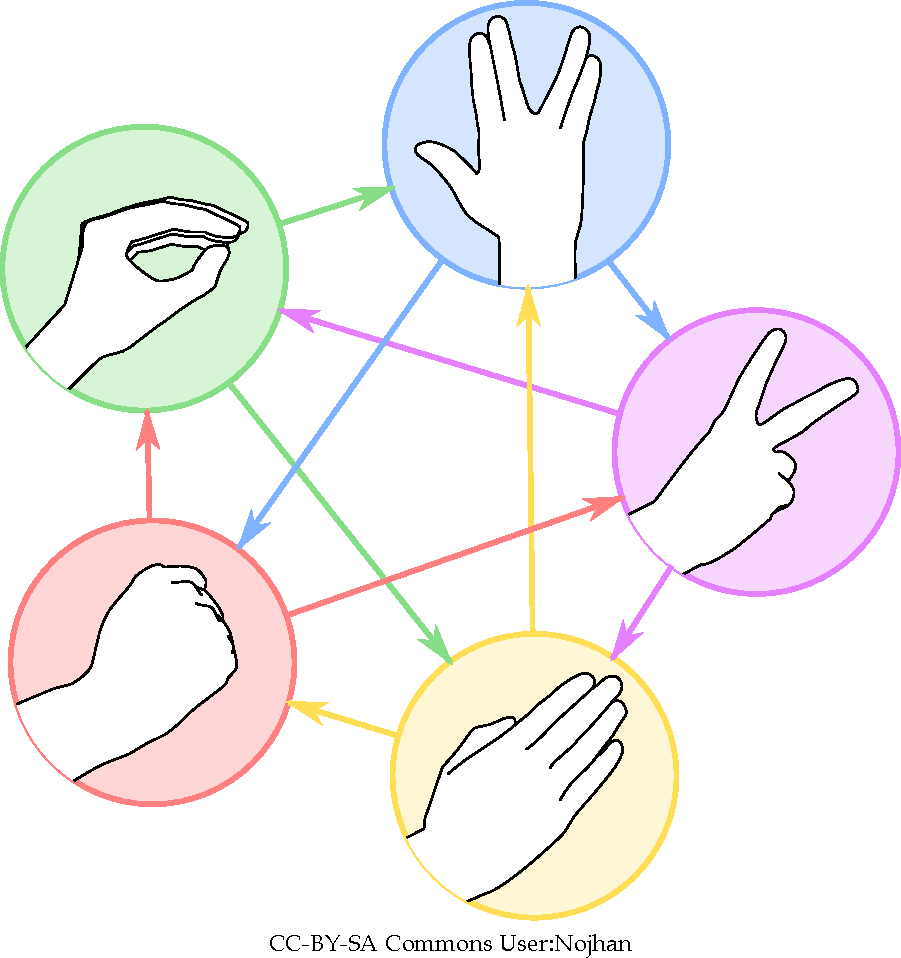
\includegraphics[width=\linewidth]{./images/rpsclsp.pdf}}
\end{minipage}
\hfill
\begin{minipage}[hbt]{0.4\linewidth}
\begin{center}
\begin{tabular}{c|ccccc}
 & R & P & Sc & L & Sp \\\hline
R & 0 & -1 & 1 & 1 & -1\\
P & 1 & 0 & -1 & -1 & 1\\
Sc & -1 & 1 & 0 & 1 & -1\\
L & -1 & 1 & -1 & 0 & 1\\
S & 1 & -1 & 1 & -1 & 0\\
\end{tabular}
\end{center}
\end{minipage}
\caption{Rock, Paper, Scissors, Lizard, Spock}
\label{Fig:rpsclsp}
\end{figure}


For each strategy there is a winning counter strategy. The players want to maximise, in case of the rowplayer, or minimise, in case of the columnplayer, the outcome. We have two terms that describe the strategies of both players

\[\max_{i\in \{R,P,S\}} \min_{j\in \{R,P,S\}} D(i,j) \qquad \min_{j\in \{R,P,S\}}\max_{i\in \{R,P,S\}} D(i,j)\]

The first term is -1, the second 1. Note that in this example it is assumed that one player makes a choice and the other player makes his move after beeing informed about this choice. This observation carries over to all games:

\begin{lem}\label{2pzsLemma1} For all game matrices $D\in R^{n\times m}$
\[\max_{i\in \{R,P,S\}} \min_{j\in \{R,P,S\}} D(i,j) \leq \min_{j\in \{R,P,S\}}\max_{i\in \{R,P,S\}} D(i,j)\]
\end{lem}

More interesting than the case of a deterministic choice of exactly one strategy is the case where randomised strategies are allowed, e.g. each player assigns a probability distribution to his available strategies.

But first let's define games formally.

\begin{Def}[2P-ZS Games] A two player zero sum game is defined by 
\begin{enumerate}
\item $S_1$, a set of strategies $n$ for player 1
\item $S_2$, a set of strategies $m$ for player 2
\item A payoff matrix $D\in R^{n\times m}$ %s.t. the sum of all rows and all columns is zero %me thinks
\end{enumerate}
\end{Def}

\begin{Def}[Mixed Strategy] A mixed strategy for player 1 is a probability distribution over $S_1$, denoted by $x\in \R^{|S_1|}, x\geq 0, \trans 1 x=1$
\end{Def}

Now we can rewrite the lemma \ref{2pzsLemma1} as follows

\begin{lem} For all 2P-ZS games we have

\[\max_x\min_y\E_{{i\sim x}\atop {j\sim y}} [D_{ij}] \leq \min_y\max_x\E_{{i\sim x}\atop {j\sim y}} [D_{ij}]\]

\end{lem}

The notation $\E_{{i\sim x}\atop {j\sim y}} [D_{ij}]$ should be understood as: 'The expected value of $D_{ij}$ with $i,j$ being choosen according to the propability distributions $x$ and $y$ '.\\ 
We can rewrite the expectations like this

\begin{align*}
\E_{{i\sim x}\atop {j\sim y}} [D_{ij}] &= \sum_{i,j} x_i D_{ij}y_j\\
	&=\sum_j y_j \left(\sum_i x_iD_{ij}\right)\\
	&=\sum_j y_j \E[x|y]
	&=\trans x D y
\end{align*}

Now we show that with mixed strategies the inequality is actually an equality

\begin{thm}[Minimax theorem] Von Neumann discovered
\[\max_x\min_y \trans xDy = \min_y\max_x \trans x Dy\]
\end{thm}

\begin{pr} We will prove this by giving two primal-dual LPs and invoking theorem \ref{thm:strongDuality}. Let

\[z^* = \max_x \min_y \trans x Dy \qquad t^*= \min_y\max_x \trans x D y\]

The LP that computes the optimal strategy for the first player is

\begin{align*}
\max \quad & z\\
s.t.\quad & z \leq \sum_{i=1}^n x_i D_{ij} & \forall j=1\ldots m\\
&\trans 1 x = 1\\
&x\geq 0
\end{align*}

This works because once the other players strategy $j$ is fixed we can just select the pure strategy that maximises our payoff. Note that the $m$ constraints of the form $z \leq \sum_{i=1}^n x_i D_{ij}, \forall j=1 \ldots m$ can be written as $z=\min_{j=1\ldots m} \sum_{i=1}^n x_i D_{ij}$.

The dual of this program is

\begin{align*}
\min \quad & t \\
s.t.\quad & \sum_{j=1}^n t-y_jD_{ij}  \geq 0 & \forall i=1\ldots n\\
& \trans 1 y = 1\\
&t \text{ free}\\
&y\geq 0
\end{align*}

Where the $y_j$ are the variables for the $z \leq \sum_{i=1}^n x_i D_{ij}$ constraints and $t$ is the variable for the $\trans 1 x=1$ constraint. 

We can rewrite the first constraint to set $t$ to the maximum of $\sum_{j=1}^n y_jD_{ij}$

\begin{align*}
\min \quad & t \\
s.t.\quad & t = \max_i \sum^m_{j=1} y_j D_{ij} & \forall i=1\ldots n\\
& \trans 1 y = 1\\
&t \text{ free}\\
&y\geq 0
\end{align*}

Which gives us the optimal mixed strategy of the second player. Because of theorem \ref{thm:strongDuality} (Strong duality) it follows that $z^{*}=t^{*}$. This implies that the optimal strategy yields a return of $0$ for both playes, as it is a zero-sum game.
\end{pr}

\subsubsection{Lower Bounds for Randomised Algorithms}

\paragraph{Problem} Given a matrix $D\in \B^{n\times n}$. We want to check whether that matrix has an all 0 column. 

Let $I$ be the set of all instances of size $n$, $A$ the set of deterministic algorithms that solve the problem and $D$ a complexity measure in $\R^{|I| \times |A|}$ that tells us the resource usage (under some measure) for each instance and each algorithm. Here we use $D[i,a]$ to denote the number of entries of $i\in I$ algorithm $a\in A$ reads.

\begin{Def} The worst-case complexity of $a\in A$ is 
\[\max_{i\in I} D(i,a)\]
\end{Def}

We want to find an algorithm that has the best possible worst case complexity, i.e.

\[a = \min_a \max_{i\in I} D(i,a)\]

Which is pretty similar to the game objectives in the previous section. Player one chooses an algorithm and player two tries to find the worst instance for it.

Fix an algorithm $a$. What is $D(i,a)$ (for any sensible $a$)? The algorithm checks the entries in some particular order, an adversary will choose a matrix such that the last entry that is checked in every column is the only '1' in it (could be any number $\neq 0$). That way the algorithm needs $n^2$ steps.

Can randomisation help? Let {\sc Rand-Check} be the algorithm that picks a random permutation of the columns and then checks that column randomly

\begin{lstlisting}
pick a random permutation $\pi$
for b = 1 $\ldots$ n
	//scan column $\pi(b)$
	for a=1 $\ldots$ n
		if $M[\pi(a),\pi(b)]=1$ break
		if $a=n$ return "yes"
return "no"
\end{lstlisting}

Since this is a randomised algorithm we want to study the expected runtime. 

\begin{Def}[Expected Runtime] The worst-case expected complexity of a randomized algorithm $a$
\[\max_{i\in I} \E[D(i,a)]\]
\end{Def}

We try to build some intuition for the structure of the worst-case instance. For this we take the view of the adversary.
It doesn't make sense to have a null column, as this would give the algorithm the chance to finish before it tried at least on element from all columns. Adding ones also makes the algorithm quit faster. Therefore let $O$ then be the set of $n\times n$ matrices with a single one value per column.

Then we have

\begin{align*}
\max_{i\in O} \E[\text{\# entries read}] &= \max_{i\in O} \sum_b \E[\text{ entries read in } i_b]\\
	&=\max_{i\in O}\sum_b \sum_{j=1}^n \frac jn\\
	&=\sum_b \frac 1n \frac{n(n+1)}{2} 
	&=\frac{n(n+1)}{2}
\end{align*}

So randomisation doesn't buy us anything. But is there a smarter algorithm than {\sc Rand-Check}? We'll prove that any randomised algorithm needs $O(n^2)$ lookups. We'll see an randomised algorithms as a probability distributions over deterministic algorithms (once we fix a sequence of random choices any randomised algorithm becomes deterministic).

We can redefine the expected runtime using this view:

\begin{Def} The worst-case expeted complexity of a probability distribution $y$ over A is
\[\max_{i\in I} \E_{a\sim y}[D(i,a)] = \max_{i\in I} \sum_{a\in A} y_a D(i,a)\]
\end{Def}

Note the similarity to mixed strategies in games. To find a bound for the runtime of the most efficient randomised algorithm we want to bound 

\[\min_y \max_i \E_{a\sim y}[D(i,a)] \geq \max_x\min_{a\in A} \E_{i\sim x}[D(i,a)]\]

That formula means that the worst case complexity of any algorithm can't be smaller than the performance of the best deterministic algorithm over the worst distribution of instances. So we need to find a distribution that is bad for any deterministic algorithm. This is different from the first case where we had a fixed algorithm and could build a tailor-made matrix to make its life hard.

Let $x$ be a probability distribution over $I$ that picks random elements in $O$ (remember: the set of matrices with one 1 per column) uniformly.

Fix an algorithm $a$ and look at $\E_{i\sim x}[D(i,u)]$. We can focus on what happens in a single column $b$, since the columns are indepedent from each other. The algorithm has to read entries in the column until it reads an one. If it checks an entry it is a one with probability $\frac{1}{n}$. The probability that it does $k$ steps is

\[\frac{1}{n} + \frac{n-1}{n}\left( \frac{1}{n-1}^2+\frac{n-2}{n-1}\left(\ldots = \frac{1}{n} + \frac 2n + \frac 3n + \right.\right.\ldots= \frac{n+1}{2}\]

So in one column we need $O(n)$, and we have $n$ of those therefore the complexity is $O(n^2)$.

